\chapter{Our Approach}\label{ourapproach}

In this chapter we have discussed our approach to solve the generalized Quorum Planted Motif Search problem. We have proposed some increment technique on some existing algorithms for solving qPMS problem more efficiently. We have also proposed the idea to implement parallelism for solving this problem.

\section{Notations and Definitions}
We have used some common notations to describe all the algorithms described and reviewed. The notations and definitions have been summarized in table \cref{notations_and_def}. The first five notations ($\Sigma, s_i, l, d, q$) are the input data of the problem. Other notations have been used in several steps the algorithms. 


%\begin{tabular}{columns}
\begin{table}
	\begin{center}
		\caption{Notations and Definitions}
		\label{notations_and_def}
		\begin{tabular}{|r|p{280 pt}|}
			\hline
			Notations & Definitions \\
			\hline
			$ \Sigma $: & The alphabet \\			
			$s_{i}$: 
			&  The input string of length $m$ over $\Sigma$ ( $1 \leq i \leq n $)\\
			$l$:
			& The motif length\\
			$d$:
			&  The maximum number of mismatches allowed in each occurrences\\
			$q$:
			& The minimum number of input strings that should have at least one occurrence.\\
			$|a|$:
			& the length of a string $a$.\\
			$a[j]$:
			&  The $j$th letter of a string $a$.\\
			$a\circ b$:
			& The string generated by concatenating two strings $a$ and $b$\\
			$d_{H}(a,b)$:
			& The Hamming distance between two strings $a$ and $b$ of the same length. It is given by the number of positions $j$ such that $a[j] \ne b[j]$\\
			$s_{ij}^{l}$:
			& The $l$-length substring of an input string $s_{i}$ that starts from the $j$th position.\\
			
			$S_{i}$: 			
			& The set of all the $l$-length substrings of an input string
			$s_{i}$. $S_{i}=\{s_{i1}^{l},...,s_{i,m−l+1}^{l}\}$.
			\\
			$S_{i}^{d}$:
			
			& The set of all the $(l+1)$-length substrings of an input string $s_{i}$ defined by $S_{i}^{d}$= \{$s_{l+1}^{i0},...,s_{i,m−l+1}^{l+1}$\}. Here, $s_{i0}^{l+1}[1] = s_{i,m-l+1}^{l+1}[l+1] = \emptyset$, and $d_{H}(\emptyset, \alpha) = \infty$ is assumed for any $\alpha$ $\epsilon$ $\Sigma$.
			\\
			$\mathcal{B}(a, R)$:
			& The set of strings in the sphere of radius $R$ centered at $a$. $\mathcal{B}(a,R)$ = $\{b$$\vert$ $\lvert b\rvert = |a|, d_{H}(a,b)\leq R$\}
			
			\\
			$n_{\mathcal{B}}(l,d)$:
			& $\lvert \mathcal{B}(a,d)\rvert$ for an $l$-length string $a$.
			\\
			$x|_{P}$:
			& The substring of $x$ composed by sequencing the letters of $x$ at the positions in a vector $P$. For example, $x|_{P}$ = GCA for $x$ = ACCGAT and $P = (4,2,5)$.\\
			$P(j)$:
			& The $j$th element of a vector $P$.\\
			$P_{+}(j)$:
 			& The $j$-dimensional vecor composed of the first $j$ elements of a vector $P$.\\
 			$P_{-}(j)$:
 			& The $(|P|-j)$-dimensional vector composed of the last $|P|-j$ elements of a vector $P$.\\
 			$R_1(a,b,c)$:
 			& The set of indices $j$ satisfying $a[j] = b[j] = c[j]$.\\
 			$R_2(a,b,c)$:
 			& The set of indices $j$ satisfying $a[j] = b[j] \neq c[j]$.\\
 			$R_3(a,b,c)$:
 			& The set of indices $j$ satisfying $c[j] = a[j] \neq b[j]$.\\
 			$R_4(a,b,c)$:
 			& The set of indices $j$ satisfying $b[j] = c[j] \neq a[j]$.\\
 			$R_5(a,b,c)$:
 			& The set of indices $j$ satisfying $a[j] \neq b[j], b[j] \neq c[j]$ and $c[j] \neq a[j]$.
 			\\ \hline
		\end{tabular}
	\end{center}
\end{table}



\section{Previous Works}
There are several exact algorithms to solve the planted motif search problem. For the sake of completeness we will describe the previous works which have motivated us to develop our approach. In this section we will review qPMSPruneI \cite{davila2007fast}, qPMS7 \cite{dinh2012qpms7}, Traver String Ref \cite{tanaka2014improved} and PMS8 \cite{nicolae2014efficient}.


\subsection{qPMSPrune}
Algorithm qPMSPrune\index{qPMSPrune} for the qPMS problem was proposed by \cite{davila2007fast}. Algorithm qPMSPrune introduces a tree structure to find the possible motif candidates. Then it uses branch-and-bound technique to reduce the search space and find the expected ($l,d$) motifs for the given set of inputs. Algorithm qPMSPrune uses the d-neighborhood concept to build the tree structure. The key points of the algorithm is described as follows.

\subsubsection{Key Steps of qPMSPruneI}
Most of the motif search algorithms combine a sample diven approach with a pattern driven approach. Here in the sample driven part the $d$-neighborhood ($\mathcal{B}(x_0,d)$) of a given input string $x_0$ is generated as a tree. Every $l$-mer in the neighborhood is a candidate motif. \\

The qPMSPrune algorithm is based on the following observation.\\

\textbf{Observation 3.1} \textit{Let M be any ($l,d,q$)-motif of the input strings $s_1,\dots,s_n$. Then there exists an $i$ (with $1\leq i\leq n-q+1$) and a $l$-mer $x\epsilon s_i^l$ such that M is in $\mathcal{B(x,d)}$ and M is a ($l,d,q-1$)-motif of the input strings excluding $s_i$.}

Based on the above observation, for any $l$-mer $x$, it represents $\mathcal{B}(x,d)$ as a tree $\mathcal{T}_{d}(x)$. It generates the $d$-neighborhood of every $l$-mer $x$ in $s_1$ by generating the tree $\mathcal{T}_{d}(x)$. The height of $\mathcal{T}_{d}(x)$ is $d$. The root of this tree will have $x$. If a node $t$ is parent of a node $t'$ then the hamming distance between the strings is $d_{H}(t,t')=1$. As a result, if a node is at level $h$, then its hamming distance from the root is $h$.\\
For example, the tree $\mathcal{T}_{2}(1010)$ with alphabet $\Sigma=\{0,1\}$ is illustrated in Figure \cref{fig:pmsprunetree}.
\\

\begin{figure}[!tb]
	\centering
	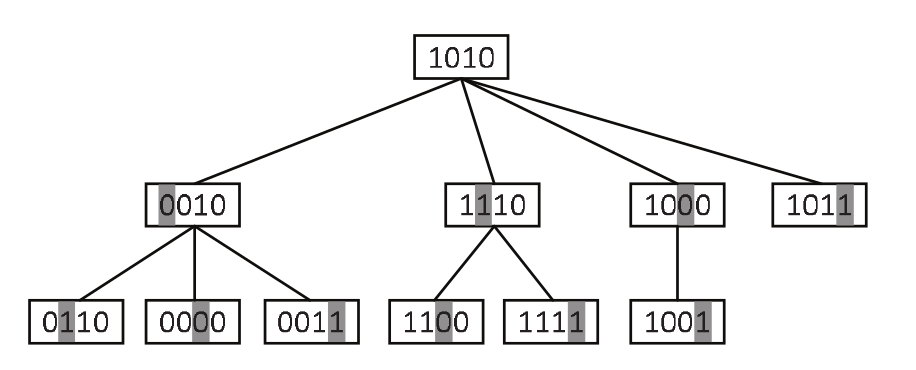
\includegraphics[width=0.9\textwidth]{figures/pmsprunetree}
	\caption{$\mathcal{T}_{2}(1010)$ with alphabet $\Sigma =\{0,1\}$}
	\label{fig:pmsprunetree}
\end{figure}

The trees are generated and explored in depth first manner. In pattern driven part, each node is checked whether it is a valid motif or not. While traversing a node $t$ in the tree $\mathcal{T}_{d}(x)$ in a depth-first manner, the hamming distance between the input strings are calculated incrementally. If $q'$ is the number of input strings $s_j$ such that $d_{H}(t,s_j)\leq d$. If $q'\geq q-1$, output $t$ as a motif. Moreover the algorithm prunes the branch if $q" < q-1$ where $q"$ is the number of input strings $s_j$ such that $d_H(t,s_j) \leq 2d-d_{H}(t,x)$.\\

The time and space complexities of algorithm qPMSPrune are given by $O((n-q+1)nm^{2}n_{\mathcal{B}}(l,d))$ and $O(nm^2)$  respectively. The pseudocode of qPMSPrune is shown in algorithm \cref{qpmsprune}.

\begin{algorithm}[H]
	\caption{qPMSPrune}
	\label{qpmsprune}
	\begin{algorithmic}[1]
		\input{algorithms/qPMSPrune.alg}
	\end{algorithmic}
\end{algorithm}

\begin{algorithm}[H]
	\caption{qPMSPrune\_Tree($k,x_{k},p_{k},\mathcal{T}$)}
	\label{qpmsprune_tree}
	\begin{algorithmic}[1]
		\input{algorithms/qPMSPrune_Tree.alg}
	\end{algorithmic}
\end{algorithm}

\begin{algorithm}[H]
	\caption{FeasibleOccurrences2($k,x_{k},\mathcal{Q}$)}
	\label{feasibleoccurrences2}
	\begin{algorithmic}[1]
		\input{algorithms/FeasibleOccurrences2.alg}
	\end{algorithmic}
\end{algorithm}

\begin{algorithm}[H]
	\caption{IsMotif($x,q',\mathcal{T}$)}
	\label{ismotif}
	\begin{algorithmic}[1]
		\input{algorithms/IsMotif.alg}
	\end{algorithmic}
\end{algorithm}


%\begin{enumerate}
%	\item Each node in $\mathcal{T}_{d}(x)$ is a pair ($t,p$) where $t=t[1]\dots t[l]$ is an $l$-mer and $p$ is an integer between 0 and $l$ such that $t[p+1]\dots t[l] = x[p+1]\dots x[l]$. A node ($t,p$) is referred to as a $l$-mer $t$ if $p$ is clear.
%	\item Let $t=t[1]\dots t[l]$ and $t'=t'[1]\dots t'[l]$. A node ($t,p$) is the parent of a node ($t',p'$) 
%\end{enumerate}

\subsection{qPMS7}
Algorithm qPMS7\index{qPMS7} was proposed by \cite{dinh2012qpms7} which was based on qPMSPrune \cite{davila2007fast}. Some speedup techniques were introduced to improve the runtime of Algorithm qPMSPrune. 
qPMS7 also searches for motifs by traversing trees. The primary difference from qPMSPrune is that it utilizes $r\epsilon \mathcal{S}_2$ as well as $x_0 \epsilon \mathcal{S}_1$ to traverse a tree. The algorithm is based on the following observations.

\textbf{Observation 3.2} Let $M$ be any ($l, d, q$)-motif of the input strings $s_1,\dots,s_n$. Then there exist $1\leq i\neq j\leq n$ and $l$-mer $x\epsilon s_{i}^{l}$ and $l$-mer $y\epsilon s_{j}^{l}$ such that $M$ is in $\mathcal{B}(x,d) \cup \mathcal{B}(y,d)$ and $M$ is a ($l, d, q-2$)-motif of the input strings excluding $s_i$ and $s_j$.\\
Using an argument similar to the one in \cite{davila2007fast}, we infer that it is enough to consider every pair of input strings $s_i$ and $s_j$ with $1\leq i,j\leq(n-q+2)$. As a result, the above observation gets strengthened as follows.\\
\textbf{Observation 3.3} Let {$M$ be any ($l,d,q$)-motif of the input strings
$s_1,\dots,s_n$. Then there exist $1\leq i\neq j\leq n-q+2$ and $l$-mer $x\epsilon s_{i}^{l}$ and $l$-mer $y\epsilon s_{j}^{l}$ such that $M$ is in $\mathcal{B}(x,d) \cup \mathcal{B}(y,d)$ and $M$ is a ($l, d, q-2$)-motif of the input strings excluding $s_i$ and $s_j$.\\

Algorithm qPMS7 uses a routine based on the above observations which finds all of the possible motifs. Algorithm qPMSPrune explores $\mathcal{B}(x,d)$ by traversing the tree $\mathcal{T}_{d}(x)$. In Algorithm qPMS7, $\mathcal{B}(x,d)\cup \mathcal{B}(y,d)$ is explored by traversing an acyclic graph, denoted as $\mathcal{G}_{d}(x,y)$ with similar constructing rule as $\mathcal{T}_{d}(x)$.


The time and space complexity of Algorithm qPMS7 are $O((n-q+1)^{2}nm^{2}
n_{\mathcal{B}}(x,d))$ and $O(nm^2)$ respectively. So in worst case scenario the time runtime of qPMS7 is worse than that of Algorithm qPMSPrune by a factor of $n-q+1$. However, Algorithm qPMS7 is much faster than Algorithm qPMSPrune in practice.


\begin{figure}[!tb]
	\centering
	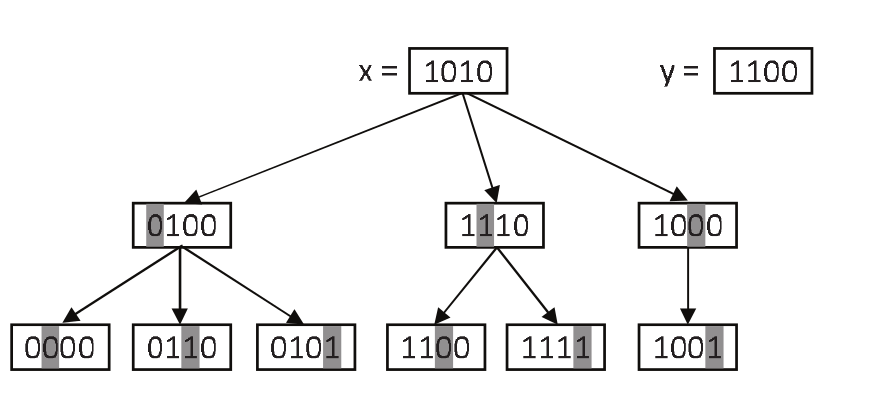
\includegraphics[width=0.9\textwidth]{figures/qpms7}
	\caption{$\mathcal{G}_{2}(1010,1100)$ with alphabet $\Sigma =\{0,1\}$}
	\label{fig:qpms7}
\end{figure}

\begin{algorithm}[H]
	\caption{qPMS7}
	\label{qpms7}
	\begin{algorithmic}[1]
		\input{algorithms/qPMS7.alg}
	\end{algorithmic}
\end{algorithm}


\begin{algorithm}[H]
	\caption{qPMS7\_Tree($k,x_{0},r,x_k,p_k,\mathcal{T}$)}
	\label{qpms7_tree}
	\begin{algorithmic}[1]
		\input{algorithms/qPMS7_Tree.alg}
	\end{algorithmic}
\end{algorithm}


\begin{algorithm}[H]
	\caption{FeasibleOccurrences3($x_0,r,x_k,p_k,\mathcal{Q}$)}
	\label{feasibleoccurrences3}
	\begin{algorithmic}[1]
		\input{algorithms/FeasibleOccurrences3.alg}
	\end{algorithmic}
\end{algorithm}


\subsection{TraverStringRef}
TraverStringRef\index{TraverStringRef} is an improved version of qPMS7. Four improvements were proposed for which will be explained below: \newline
	
\subsubsection{Feasibility Check without Precomputed Table}
Like qPMS7 feasibility check is not performed by checking an occurrnce in the precomputed table. Here a theorem is followed:
Three strings $a,b,c$ of the same length satisfy
\begin{center}
	$\mathcal{B}(a,d_{a})\cap \mathcal{B}(b,d_{b})\cap \mathcal{B}(c,d_{c})\neq \emptyset$
\end{center}
if and only if 
\begin{center}
	$d_{a} \geq 0, d_{b} \geq 0, d_{c} \geq 0, \newline d_{a}+d_{b} \geq d_{H}(a,b), \newline d_{b}+d_{c} \geq d_{H}(b,c), \newline d_{c}+d_{a} \geq d_{H}(c,a), \newline d_{a}+d_{b}+d_{c} \geq |R_{2}(a,b,c)|+ |R_{3}(a,b,c)|+ |R_{4}(a,b,c)|+ |R_{5}(a,b,c)|$
	
\end{center}	


\subsubsection{Elimination of unnecessary Combinations}
Unnecessary combinations are eliminated in qPMS7 and the procedure is quite same as qPMSPruneI. The unnecessary checks are suppressed when $q<n$ and $\mathcal{T} \leftarrow \{S_{h}|i_{2}+1 \leq h \leq n\}$.

\subsubsection{String Reordering}
This improvement is ensured by pruning the subtree rooted at current node as early as possible by checking the feasibility occurences in non decreasing order. Here the difference is when the input string from where the input reference occurences are taken is determined. Since the number of string in $\mathcal{B}(x_{0},d) \cap \mathcal{B}(r,d)$ is a non decreasing function of $d_{H}(x_{0},r)$ the reference $r$ is taken from the input that maximizes minimum hammimg distance between $x_{0}$ and $r$ to reduce size of the search tree.

\subsubsection{Position Reordering}
To ensure efficient pruning of subtrees the search tree's structure is investigated. Only the nodes satisfying the condition of not changing the hamming distance change the structure of the search tree. To take the advantage of this procedure the position of the strings reordered so that the positions where the letters are different come earlier. For this an $l$-dimensional vector is computed for each pair at the root node of the search tree.\\


The pseudo-code of the algorithm TraverStringRef is given in Algorithm [\cref{traver_string_ref}].

\begin{algorithm}[H]
	\caption{TraverStringRef}
	\label{traver_string_ref}
	\begin{algorithmic}[1]
		\input{algorithms/TraverStringRef.alg}
	\end{algorithmic}
\end{algorithm}

\begin{algorithm}[H]
	\caption{TraverStringRef\_Tree($k,x_0,r,x_k,p_k,\mathcal{T},J$)}
	\label{traver_string_ref_tree}
	\begin{algorithmic}[1]
		\input{algorithms/TraverStringRef_Tree.alg}
	\end{algorithmic}
\end{algorithm}

\subsection{PMS8}
The key concepts of increasing efficiency in PMS8\index{PMS8} from qPMS7 and qPMSPrune are described below:

\subsubsection{Sort rows by size}
Sorted rows speed up the filtering step. As for sorted rows we need less tuples for lower stack size, it helps to reduce expensive filtering. It is because fewer $l$-mers remain to be filtered when the stack size increases.

\subsubsection{Compress $l$-mers}
To calculate the hamming distance between two $l$-mers at first we have to perform exclusive or of their compressed representation. One compressed $l$-mer requires l $\times \lceil\log|\varSigma|\rceil$ bits of storage. So the table of compressed $l$-mers only requires O(n(m-l+1)) words of memory as we only need the first 16 bit of this representation.

\subsubsection{Preprocess distances for pairs of $l$-mers}
For every pair of $l$-mers we test if the distance is no more than 2d in advance.

\subsubsection{Cache locality}
As a certain row of an updated matrix is the subset of that row so we can store the updated row in the previous location of the row. so we have to keep track the number of elements belongs to the new row. This process can be repeated in every step of recursion and can be perform using by only a single stack where the subset elements are in contiguous position of memories and thus cache locality sustains.

\subsubsection{Find motifs for a subset of strings}
we will find the motif for some input strings and then test them against the remaining strings.

\subsubsection{Memory and Runtime}
since we store all the matrices in the place of a single matrix they only require $O(n(n-l+1))$ words of memory. $O(n^2)$ words of row size will be added for at most n matrices which share the same space. So total bits of $l$-mer pair takes $O((n(m-l+1)^2)/w)$ words where w is the number of bits in a machine word. So total memory used for this algorithm is $O(n(n-l+1)+(n(m-l+1)^2)/w)$.

\subsubsection{Parallel implementation}
If we think dividing the problem into $m-l+1$ subproblems then the number of subproblems will be embarrassingly greater for parallelization. So a fixed number of subproblems are assigned to each processor. Scheduler then spawns a separate worker thread to avoid use of a processor just for scheduling. The scheduler loops until all the subproblems are solved and after the completion of all threads the motifs are given to scheduler and it outputs the result.

%\subsubsection{Pruning conditions}
%For two $l$-mers a and b the pruning condition is given below: \newline a and b have a common neighbor M such that $H_{d}(a,M) \leq d_{a}$ and $H_{d}(b,M) \leq d_{b}$ if and only if $H_{d}(a,b) \leq d_{a}+d_{b}.$


\section{Our Proposal qPMS-Sigma}
In this section we propose an algorithm qPMS-Sigma with some techniques to optimize the space complexity as well as the runtime to solve the Quorum Planted Motif Search problem. Our work is mainly based on the Algorithm TraverStringRef. 

\subsection{String Compression}\index{Compression}
We can compress the input strings $s_1,\dots s_n$ as a part of preprocessing of the algorithm. For our work we have compressed all the $l$-mers of the input strings into some group of unsigned 32-bit integers. Thus we make the motif matrix using the compressed $l$-mers. To be specific for an alphabet set $\Sigma$ we compressed a $l$-mer into $\lceil \log_{2}(\lvert \Sigma \rvert)\rceil$ groups. Each of this group contains $\lceil l/32\rceil$ 32-integers. \\

For example, for a DNA string of 32 characters, we need $\lceil \log_{2}(\lvert \Sigma \rvert)\rceil=2$ groups of unsigned 32-bit integers,  where each group contains $\lceil n/32\rceil = 1$ integers.\\

We can calculate the hamming distance between two compressed $l$-mers in two steps. First for each group of integers find out the bitwise XOR values of the integers of both the $l$-mers. After that calculate the bitwise OR values among the XOR-ed values of each group. The number of set bits in the last set of integers is the hamming distance between the two strings.\\

An example of comparing two compressed $l$-mers is given in \cref{strexample}.

\begin{figure}[H]
	\centering
	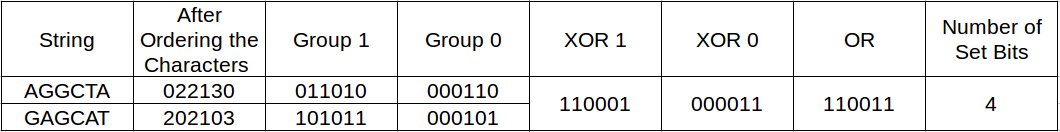
\includegraphics[width=0.9\textwidth]{figures/example.png}
	\caption{$l$-mer Compression Example}
	\label{strexample}
\end{figure}

%\begin{table}[H]
%	\begin{center}
%		\caption{Compression Example}
%		\label{strexample}
%		\begin{tabular}{|c|c|c|c|c|c|c|c|}
%			\hline
%			String & After Ordering the Characters & $Group_{1}$ & $Group_{0}$ & $XOR_{1}$ & $XOR_{0}$ & OR & SetBits\\
%			\hline
%			AGGCTA & 022130 & 011010 & 000110 & 110001 & 000011 & 110011 & 4 \\
%			\hline
%			GAGCAT & 202103 & 101011 & 000101 & & & & \\ \hline
%		\end{tabular}
%	\end{center}
%\end{table}

A code snippet \cref{string_compress} is written in C++ describing the structure of compressed $l$-mer and the method of calculating hamming distance.\\

%After compressing the input strings we can calculate the hamming distance between two l-mers in $O(l/(w/\log_{2}\Sigma))$, where $W$ is the size of the integer, which is 32 in our experiment.

\subsection{Motif Finding}
After compressing the input sequences we need to find the motifs in them. For these we've modified the TraverStringRef algorithm by using the compressed $l$-mers. Then we have followed the steps of Algorithm TraverStringRef \index{TraverStringRef} to find out the motifs.

\subsection{Parallel Implementation of qPMS-Sigma}\index{Parallel}
The Algorithm qPMS-Sigma can easily implement in parallel by traversing several search trees in parallel. Similar to the idea of parallelism mentioned in Algorithm TraverStringRef \cite{tanaka2014improved} we can divide the problem into $(m-l+1)$ subproblem where each subproblem explores different search trees.



\section{Space and Runtime Complexity}
Here the space complexity\index{space complexity} of our algorithm is $O(nml(\log \lceil \Sigma \rceil)/w)$. Here $w$ is the size of the integers that contain the compressed  input sequences as well as the $l$-mers. For DNA sequences $\log \lvert \Sigma \rvert = 2$. So the space complexity becomes $O(nml/w)$.\\

The worst case time complexity is similar to TraverStringRef $O((n-q+1)^2 nm^2 (m+\log n)n_\mathcal{B} (l,d))$. However, finding the hamming distance between two $l$-mers take about constant time for DNA sequence. Normally bitwise operations are a little faster than the other arithmetic operations. So, practically our algorithm runs a little faster than the former.

\section{Experimental Results}
We have compared the runtime of Algorithm qPMS-Sigma in the challenging states with the other well known algorithms. The proposed algorithm is implemented in C++ (using GNU C++ compiler). We have run the experiment on Ubuntu 14.04 (64 bit) operating system. The machine configuration is Intel\textregistered Core\texttrademark i3-4005U CPU @ 1.70GHz × 4, 4GB RAM.

The test dataset was generated in computational experiment of Algorithm TraverStringRef \cite{tanaka2014improved}. The testing dataset is randomly generated according to the FM (fixed number of mutation) model \cite{pevzner2000combinatorial}. We have used it in our experiment and showed the result in \cref{dataq20} and \cref{dataq10}. Our algorithm shows a little better result than Algorithm TraverStringRef in some challenging
states. Although it lags behind the qPMS9 in all cases. The comparisons are shown in \cref{dataq20}, \cref{dataq10}, \cref{fig:chart1}, \cref{fig:chart2}.

\begin{table}
	\begin{center}
		\caption{Parameter Setting for Testing Data Set}
		\label{dataset_parameter}
		\begin{tabular}{|ll|}
			\hline 
			Parameter
			& Setting\\
			\hline
			$|\Sigma|$
			& 4 (DNA)\\
			$n$
			& 20 \\
			$m$
			& 600 \\
			$q$
			& 10,20\\
			$l$
			& 13, 15, 17,\dots \\
			\hline
		\end{tabular}
	\end{center}
\end{table}

\begin{table}
	\begin{center}
		\caption{Computational Results for DNA Sequences for $q=20$}
		\label{dataq20}
		\begin{tabular}{|c|c|c|c|c|c|c|}
			\hline 
			\textbf{Algorithm} & \textbf{(13,4)} & \textbf{(15,5)} & \textbf{(17,6)} & \textbf{(19,7)} & \textbf{(21,8)} & \textbf{(23,9)} \\
			\hline
			\textbf{qPMS-Sigma} & 12s & 50s & 165s & 755s & 2909s & 12153s \\
			\hline
			\textbf{TraverStringRef} & 11s & 47s & 179s & 745s & 3098s & 13027s \\
			\hline
			\textbf{qPMS7} & 14s & 133s & 1046s & 8465s & 71749s & \\ \hline
			\textbf{PMS8} & 7s & 48s & 312s & 1596s & 5904s & 19728s\\ \hline
			\textbf{qPMS9} & 6s & 34s & 162s & 804s & 2724s & 8136s \\ \hline
		\end{tabular}
	\end{center}
\end{table}
\begin{figure}[!tb]
	\centering
	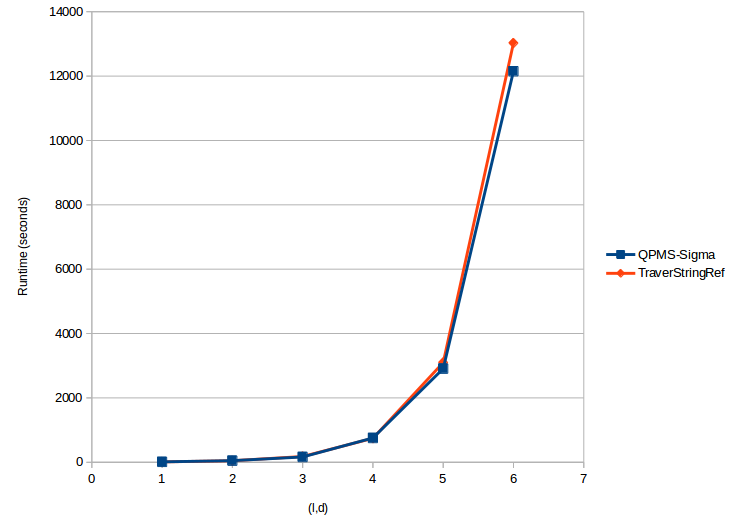
\includegraphics[width=0.9\textwidth]{figures/chart1.png}
	\caption{Run Time Comparison between qPMS-Sigma vs TraverStringRef in the challenging states for q=20}
	\label{fig:chart1}
\end{figure}

\begin{table}
	\begin{center}
		\caption{Computational Results for DNA Sequences for $q=10$}
		\label{dataq10}
		\begin{tabular}{|c|c|c|c|c|c|c|}
			\hline 
			\textbf{Algorithm} & \textbf{(13,4)} & \textbf{(15,5)} & \textbf{(17,6)} & \textbf{(19,7)} & \textbf{(21,8)} & \textbf{(23,9)} \\
			\hline
			\textbf{TraverStringRef} & 7 & 36 & 160 & 760.6 & 3643.3 & 17232.4 \\
			\hline
			\textbf{TraverStringRef} & 5.5 & 32 & 166.1 & 779.9 & 3700.6 & 17922.2 \\
			\hline
			\textbf{qPMS7} & 31 & 152 & 850.7 & & 4865.0 & 29358 \\ \hline
			\textbf{qPMSPrune} & 12.8 & 126.7 & 1116.5 & 10540.8 & & \\ \hline
			\textbf{PMS9} & & & & & & \\ \hline			
		\end{tabular}
	\end{center}
\end{table}

\begin{figure}[!tb]
	\centering
	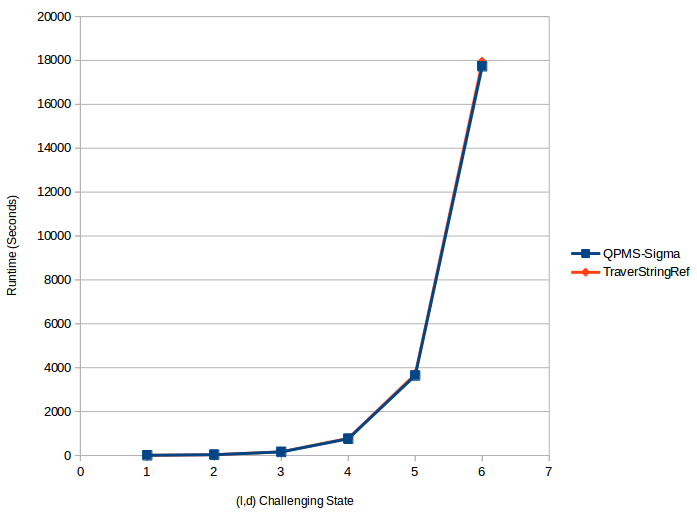
\includegraphics[width=0.9\textwidth]{figures/chart2.png}
	\caption{Run Time Comparison between qPMS-Sigma vs TraverStringRef in the challenging states for q=10}
	\label{fig:chart2}
\end{figure}